\subsection{Person 1 – SUS 67{,}5}
\textbf{Zur Person:}\\
ICompetence-Student, 27 Jahre alt\\

\textbf{Beobachtung:}
\begin{enumerate}
    \item Zeichnen Sie frei für etwa 2 Minuten.
    \begin{itemize}
        \item Nutzer wollte den «Rotate»-Button verwenden, um eine Aktion rückgängig zu machen.
        \item Handhabung des Stifts wurde als gewöhnungsbedürftig empfunden.
        \item Erkenntnis, dass die Kamera nicht zuverlässig erfasst, wenn die Hand den Stift verdeckt.
        \item Bessere Erkennung, wenn der Stift weiter hinten gehalten wird – jedoch ungewohnt.
        \item Positives Feedback: «Fühlt sich wie ein Stift an, wenn es funktioniert.»
        \item Unsicherheit, wie vorzugehen ist, wenn Striche nicht korrekt erkannt werden.
        \item Wunsch nach einem dünneren, spitzeren Stift für präziseres Zeichnen.
    \end{itemize}

    \item Löschen Sie Ihre Zeichnung vollständig.
    \begin{itemize}
        \item «Rotation»-Button wurde mit «Rückgängig»-Button verwechselt.
    \end{itemize}

    \item Laden Sie die PDF-Datei mit dem Grundriss \texttt{Hospital\_Floor\_Plan.pdf} hoch.
    \begin{itemize}
        \item Versuch, Text einzugeben anstatt eine Datei auszuwählen.
        \item PDF-Icon mit Pfeil nach aussen wurde als «Exportieren»-Symbol interpretiert.
    \end{itemize}

    \item Ändern Sie die Stiftfarbe auf Rot.
    \begin{itemize}
        \item Unklar, wo die Funktion zu finden ist.
        \item Slider zur Farbauswahl wurde bewegt, jedoch mit Problemen.
    \end{itemize}

    \item Suchen Sie \texttt{BEDROOM3} und zeichnen Sie einen Tisch links vom Bett.
    \begin{itemize}
        \item Architekt gab an, dass diese Position nicht möglich ist.
    \end{itemize}

    \item Radieren Sie den Tisch und zeichnen Sie ihn rechts vom Bett.
    \begin{itemize}
        \item Unsicherheit, ob der Radiergummi-Modus aktiviert war.
    \end{itemize}

    \item Zeichnen Sie die Abmessungen 1\,m $\times$ 1\,m und schreiben Sie «table» hinein.
    \begin{itemize}
        \item Zoom wird als nicht optimal beschrieben, vermutlich nicht genutzt.
        \item Verschiebung (Pan) nur in kleinen und langsamen Schritten möglich.
        \item Versuch, durch Gedrückthalten zu verschieben.
    \end{itemize}

    \item Speichern Sie den Plan auf Ihrem Laptop.
    \begin{itemize}
        \item Kein Dateiname angegeben, daher Standardname verwendet.
        \item Speichervorgang ohne Rückmeldung – Bestätigung (z. B. Balken mit «Saved» oder Ordner-Öffnen-Option) wäre wünschenswert.
    \end{itemize}
\end{enumerate}

\clearpage

\textbf{SUS-Antworten:}
\begin{center}
    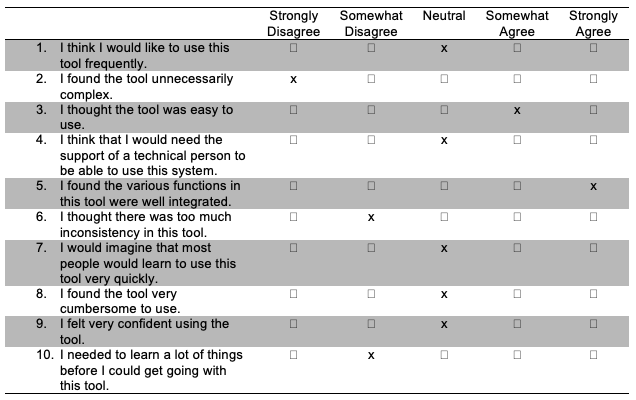
\includegraphics[width=0.95\textwidth]{graphics/sus_person1.png}
\end{center}

\textbf{Follow-up:}
\begin{enumerate}
    \item \textbf{Was hat Ihnen am Tool am besten gefallen?}
    \begin{itemize}
        \item Möglichkeit, PDF-Dateien hochzuladen und zu bearbeiten.
        \item Farb- und Stiftdickenänderung möglich.
        \item Speichern der Arbeit.
    \end{itemize}

    \item \textbf{Gab es etwas, das verwirrend oder schwierig zu bedienen war?}
    \begin{itemize}
        \item Verständnis der Zeichenfunktion.
    \end{itemize}

    \item \textbf{Fehlt etwas, das Sie erwartet oder gerne gehabt hätten?}
    \begin{itemize}
        \item Undo-Button.
        \item Speichern mit klarer Bestätigung, dass die Datei gesichert wurde.
        \item PDF-Icon nicht eindeutig.
    \end{itemize}

    \item \textbf{Haben Sie Vorschläge, wie das Tool verbessert werden könnte?}
    \begin{itemize}
        \item Anpassung der Kameraposition für besseres Zeichnen.
        \item Blaue Farbe wirkt wie Schwarz.
        \item Beim Verschieben des Plans wird auch die Zeichnung verschoben.
        \item Zusätzlicher Button für schnellen Farbwechsel.
    \end{itemize}
\end{enumerate}
\clearpage